% =====================================================================
%  Shell Eco-marathon Poland 2026 — Data & Telemetry Award (Art. 247)
%  Sponsored by Schmid Elektronik
%  Team: ThaiGer H2 Racing — Prototype · Hydrogen fuel cell
%
%  ENGINE: pdflatex  (run TWICE — second pass fixes page numbers)
%  BUILD:  pdflatex SEM-Poland-2026_DataTelemetry_APPLICATION-FINAL.tex
%          pdflatex SEM-Poland-2026_DataTelemetry_APPLICATION-FINAL.tex
%
%  HARD RULES (auto-checked — violating = disqualified without notice):
%    ≤ 10 pages ALL-inclusive (cover, tables, refs, appendices count)
%    ≥ 10 pt font size everywhere that prints
%    Team ID + Team name on cover AND in header of every page
%    No personal names or contact details anywhere
%
% ═══════════════════════════════════════════════════════════════════════
%  FILL BEFORE SUBMITTING — edit the two lines immediately below
%  (Find your Team ID and Team Name in the SEM registration portal)
% ═══════════════════════════════════════════════════════════════════════
%  Step 1: Replace \ph{Team Name} with your registered team name
%  Step 2: Replace \ph{Team ID}   with your SEM team ID number
%  Step 3: Replace \ph{date}      with the submission date
%  Step 4: pdflatex twice, verify PDF ≤ 10 pages, submit
% =====================================================================
\documentclass[11pt,a4paper]{article}

\newif\ifscaffold
\scaffoldfalse   % ← keep false for the final submission
                 %   set true to show guidance notes during drafting

\usepackage[T1]{fontenc}
\usepackage[utf8]{inputenc}
\usepackage[scaled=0.96]{helvet}
\renewcommand{\familydefault}{\sfdefault}
\usepackage[a4paper,top=18mm,bottom=18mm,left=22mm,right=22mm]{geometry}
\usepackage{microtype}
\usepackage{textcomp}
\usepackage{caption}
\usepackage{amsmath}
\usepackage{xcolor}
\usepackage{graphicx}
\usepackage{titlesec}
\usepackage{booktabs}
\usepackage{tabularx}
\usepackage{array}
\usepackage{enumitem}
\usepackage{fancyhdr}
\usepackage{lastpage}
\usepackage{needspace}
\usepackage{tcolorbox}
\tcbuselibrary{skins,raster,breakable}
\usepackage{tikz}
\usetikzlibrary{positioning,arrows.meta,calc,backgrounds}
\usepackage[hidelinks]{hyperref}

% ── Colour palette ──────────────────────────────────────────────────
\definecolor{ink}{HTML}{14181C}
\definecolor{graphite}{HTML}{585F66}
\definecolor{mist}{HTML}{C9CDD2}
\definecolor{fog}{HTML}{F2F3F5}
\definecolor{accent}{HTML}{C1121F}      % Swiss red
\colorlet{placeholdercol}{accent}
\definecolor{exdata}{HTML}{1F5AA8}      % blue for exemplary values

% ── Typography & spacing ────────────────────────────────────────────
\setlength{\parindent}{0pt}\setlength{\parskip}{0.42em}
\linespread{1.03}\color{ink}\hyphenpenalty=2000\hbadness=10000
\setlength{\emergencystretch}{2.5em}

% ── Macros ──────────────────────────────────────────────────────────
\newcommand{\tenpt}{\fontsize{10}{12}\selectfont}
\newcommand{\kicker}[1]{{\tenpt\color{graphite}\textls[150]{\MakeUppercase{#1}}}}
\newcommand{\ph}[1]{{\color{placeholdercol}\itshape[\,#1\,]}}
\newcommand{\ex}[1]{{\color{exdata}\ensuremath{\diamond}\,#1}}
\newcommand{\hyd}{H\textsubscript{2}}
\newcommand{\kmM}{km/m\textsuperscript{3}}
\newcommand{\TEAMNAME}{\ph{Team Name}}   % ← FILL THIS IN
\newcommand{\TEAMID}{\ph{Team ID}}       % ← FILL THIS IN
\newcommand{\question}[1]{\vspace{-0.15em}%
  {\tenpt\color{graphite}\itshape Rules Art.~247 asks: #1}\par\vspace{0.3em}}
\newcommand{\kpi}[2]{{\fontsize{16}{18}\selectfont\bfseries\color{ink}#1}\\[2pt]
  {\tenpt\color{graphite}\textls[40]{\MakeUppercase{#2}}}}
\newcommand{\figslot}[2]{\begin{tcolorbox}[enhanced,sharp corners,colback=fog,
  boxrule=0pt,frame hidden,height=#1,halign=center,valign=center,
  borderline={0.6pt}{0pt}{mist,dashed}]%
  {\tenpt\color{graphite}\itshape FIGURE SLOT — #2}\end{tcolorbox}}
\newcommand{\hdr}[1]{{\tenpt\color{graphite}\textls[40]{\MakeUppercase{#1}}}}

% ── tcolorbox styles ────────────────────────────────────────────────
\tcbset{
  swisspanel/.style={enhanced,sharp corners,colback=fog,boxrule=0pt,frame hidden,
    borderline north={1.4pt}{0pt}{accent},left=4mm,right=4mm,top=1.8mm,bottom=1.8mm},
  rulepanel/.style={enhanced,sharp corners,colback=white,boxrule=0pt,frame hidden,
    borderline north={0.6pt}{0pt}{mist},borderline south={0.6pt}{0pt}{mist},
    left=0mm,right=0mm,top=1.8mm,bottom=1.8mm},
  codepanel/.style={enhanced,sharp corners,colback=fog,boxrule=0pt,frame hidden,
    borderline west={2pt}{0pt}{accent},left=6mm,right=4mm,top=1.5mm,bottom=1.5mm,
    fontupper=\ttfamily\tenpt\color{ink}}
}

% ── Table column types ──────────────────────────────────────────────
\newcolumntype{L}{>{\raggedright\arraybackslash}X}
\newcolumntype{R}{>{\raggedleft\arraybackslash}X}

% ── Section heading style ───────────────────────────────────────────
\titleformat{\section}[block]
  {\needspace{4\baselineskip}\sffamily\large\bfseries\color{ink}}
  {\makebox[1.7em][l]{\color{accent}\thesection}}{0pt}{}
  [{\vspace{2pt}\color{mist}\titlerule[0.6pt]}]
\titlespacing*{\section}{0pt}{1.1em}{0.35em}
\titleformat{\subsection}[hang]{\sffamily\normalsize\bfseries\color{ink}}
  {\color{accent}\thesubsection}{0.6em}{}
\titlespacing*{\subsection}{0pt}{0.65em}{0.1em}

% ── Page headers & footers ──────────────────────────────────────────
\pagestyle{fancy}\fancyhf{}
\renewcommand{\headrulewidth}{0pt}\renewcommand{\footrulewidth}{0pt}
\fancyhead[L]{\tenpt\color{graphite}\TEAMNAME\ \ \textbullet\ \ \TEAMID}
\fancyhead[R]{\tenpt\color{graphite}\textls[80]{\MakeUppercase{Data \& Telemetry Award}}}
\fancyfoot[L]{\tenpt\color{graphite}\textls[80]{\MakeUppercase{SEM Poland 2026}}}
\fancyfoot[R]{\tenpt\color{graphite}\textcolor{accent}{\rule[-0.1ex]{1.3ex}{1.3ex}}\hspace{0.5em}\thepage\,/\,\pageref*{LastPage}}
\fancypagestyle{coverpg}{\fancyhf{}\renewcommand{\headrulewidth}{0pt}%
  \fancyfoot[R]{\tenpt\color{graphite}\textcolor{accent}{\rule[-0.1ex]{1.3ex}{1.3ex}}\hspace{0.5em}\thepage\,/\,\pageref*{LastPage}}}

% ────────────────────────────────────────────────────────────────────
\begin{document}\thispagestyle{coverpg}

% ══════════════════════════════ COVER ════════════════════════════════
\noindent{\color{ink}\rule{\linewidth}{1.2pt}}\par\vspace{3pt}
\kicker{Shell Eco-marathon Poland 2026 \ \textbullet\ \ Off-Track Award \ \textbullet\ \ Article 247}
\vspace{0.55cm}

\noindent{\fontsize{28}{31}\selectfont\color{ink}Data \& Telemetry Award}\par
\vspace{3pt}
\noindent{\fontsize{12.5}{15}\selectfont\color{graphite}sponsored by Schmid Elektronik}\par
\vspace{6pt}\noindent{\color{accent}\rule{7cm}{2pt}}\par\vspace{7pt}

\noindent{\tenpt
\begin{tabularx}{\linewidth}{@{}l L l L@{}}
\kicker{Team}        & \TEAMNAME                 & \kicker{Category}       & Prototype\\[3pt]
\kicker{Team ID}     & \TEAMID                   & \kicker{Powertrain}     & \hyd\ fuel cell + supercapacitor\\[3pt]
\kicker{Institution} & Hochschule Stralsund (DE) & \kicker{Energy sensors} & Joulemeter + Gas Flowmeter\\[3pt]
\kicker{Vehicle}     & Thaiger~7                 & \kicker{Event}          & 24--28~June~2026, Silesia~Ring\\[3pt]
\kicker{Submitted}   & \ph{date}                 & \kicker{Pages}          & $\leq$10 (Art.~245/246)\\
\end{tabularx}}\par
\vspace{5pt}\noindent{\color{mist}\rule{\linewidth}{0.6pt}}\par\vspace{4pt}

\noindent\kicker{The multi-objective racing problem — three goals (Art.~247a)}\par\vspace{3pt}
\begin{tcbraster}[raster columns=3,raster column skip=3mm,raster equal height,
  raster every box/.style={swisspanel,valign=top}]
  \begin{tcolorbox}{\bfseries\color{ink}1\ \ Terrain}\\[1pt]
    {\tenpt\color{graphite}Straights, slopes, crests \& corners mastered per segment.}\end{tcolorbox}
  \begin{tcolorbox}{\bfseries\color{ink}2\ \ Efficiency $\times$ time}\\[1pt]
    {\tenpt\color{graphite}Minimum \hyd\ at a competitive, valid lap time.}\end{tcolorbox}
  \begin{tcolorbox}{\bfseries\color{ink}3\ \ Safety always}\\[1pt]
    {\tenpt\color{graphite}Advisory-only cues; rain \& wind tighten constraints first.}\end{tcolorbox}
\end{tcbraster}
\vspace{2pt}
\noindent{\tenpt\color{graphite}%
\textls[60]{\MakeUppercase{Eligibility}}\quad
This team will have passed Technical \& Safety Inspection (Art.~247b).\hfill
\textcolor{exdata}{$\diamond$\,=\,exemplary value — replace with measured data before final submission.}}

% ═══════════════════════ EXECUTIVE SUMMARY ═══════════════════════════
\section*{Executive summary}

Thaiger~7 carries a fully self-built, working telemetry chain (v1): an ESP32
sensor hub streams 21 powertrain and motion channels over Bluetooth Low
Energy to an Android onboard computer, which relays them at 5\,Hz over
encrypted MQTT to a cloud broker and a real-time pit dashboard — all in
production today at \url{github.com/D0mm3c/ThaiGerTrackControl}.

This season we add the missing layer (v2): a \textbf{strategy engine} that
turns that data into an energy-optimal, weather-adaptive lap plan,
recomputed after every lap and delivered to the driver as three glanceable
cues. A physics model of the vehicle, identified from our own coast-down and
powertrain logs, feeds a dynamic-programming optimiser that chooses
burn/coast switching points and fuel-cell set-points per track segment,
subject to lap-time, corner-grip, temperature and minimum-speed constraints.
In simulation back-tests the optimised plan uses \ex{18\,\%} less hydrogen
than our constant-speed baseline at an average speed \ex{0.4\,km/h} higher,
with a \ex{$+$9\,s} margin to the lap-time limit.

The driver sees one decision at a time; safety alarms stay local and override
everything. \textit{All interface screenshots in this document are generated
in Demo Mode using the exemplary model; strategy numbers are simulation
back-tests against our own vehicle model. No data is presented as measured
that is not measured — consistent with Art.~245 and sound engineering
practice.}

\vspace{0.25em}
\begin{tcbraster}[raster columns=3,raster column skip=3mm,raster equal height,
  raster every box/.style={swisspanel,halign=left,valign=center}]
  \begin{tcolorbox}\kpi{\ex{$-$18\,\%}}{Hydrogen / lap}\end{tcolorbox}
  \begin{tcolorbox}\kpi{\ex{$+$1.5\,\%}}{Avg.\ speed}\end{tcolorbox}
  \begin{tcolorbox}\kpi{\ex{$+$9\,s}}{Lap-time margin}\end{tcolorbox}
\end{tcbraster}

% ═══════════════════════ SECTION 1 ════════════════════════════════════
\section{Data strategy to achieve the three goals}
\question{your overall data strategy, and which driver, vehicle and context
parameters are relevant to achieving the three goals.}

Our strategy: \textbf{measure the energy path end-to-end, locate the car on a
segmented track model, and let every captured signal either tune the vehicle
model or trigger a driver decision.} Signals that serve neither purpose are
logged but not streamed live.

\renewcommand{\arraystretch}{1.18}
\noindent\begin{tabularx}{\linewidth}{@{}>{\bfseries}l L l c@{}}
\toprule
\hdr{Group} & \hdr{Parameter — decision it drives} & \hdr{Source} & \hdr{Goal}\\
\midrule
Driver  & Mass per run (incl.\ driver + gear) — model mass $m$ & weigh per run & 1--3\\
Driver  & Cue compliance — plan realism estimate & speed vs.\ plan band & 2,3\\
Vehicle & Speed, avg.\ speed, lap count, total time — pace \& validity & wheel sensor (ESP32) & 2\\
Vehicle & FC / supercap / motor voltage \& current — operating point, buffer & shunts (ESP32) & 2\\
Vehicle & FC temperature, cell diff., air-pump duty — derating \& safety & stack sensors (ESP32) & 3\\
Vehicle & Cumulative FC / motor energy, system efficiency — energy ledger & ESP32 integration & 2\\
Vehicle & \hyd\ mass flow — true fuel ledger (replaces estimate) & \textbf{Gas Flowmeter (Schmid)} & 2\\
Context & Position, heading — segment ID, cue timing (``coast in 50\,m'') & phone GPS at 1\,Hz & 1\\
Context & Gradient, curvature per segment — terrain tactic & surveyed track model & 1\\
Context & Wind speed/direction, rain, temperature — drag, grip, air density & Open-Meteo + on-site obs. & 1, 3\\
\bottomrule
\end{tabularx}
\renewcommand{\arraystretch}{1.0}

% ═══════════════════════ SECTION 2 ════════════════════════════════════
\section{Capturing data with a telemetry system}
\question{the design of your system for near-real-time capture; hardware \&
software concept of the onboard computer; what you build in-house; and what
technology, sensors or training you need from Schmid Elektronik.}

\subsection{Architecture (built and operating today)}

\begin{figure}[h]\centering
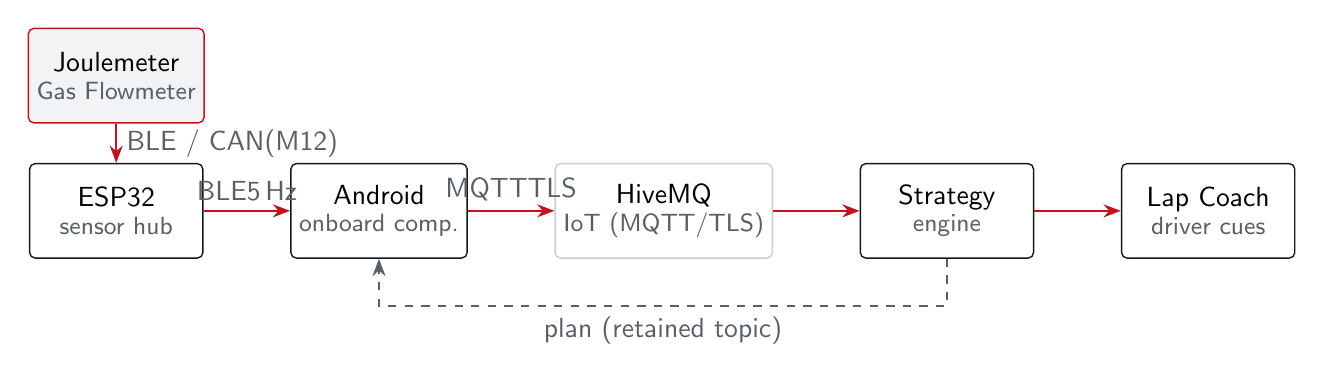
\begin{tikzpicture}[font=\fontsize{10}{11}\selectfont,
   box/.style={draw=ink,line width=0.5pt,rounded corners=2pt,
     minimum height=12mm,minimum width=22mm,align=center,inner sep=3pt},
   sensor/.style={box,draw=accent,fill=fog},
   cloud/.style={box,draw=mist,fill=white},
   flow/.style={-{Stealth[length=2.2mm]},draw=accent,line width=0.8pt},
   note/.style={font=\fontsize{10}{11}\selectfont,color=graphite}]
 \node[sensor] (j) {Joulemeter\\[-1pt]\textcolor{graphite}{\small Gas Flowmeter}};
 \node[box,below=5mm of j] (e) {ESP32\\[-1pt]\textcolor{graphite}{\small sensor hub}};
 \node[box,right=11mm of e]  (o) {Android\\[-1pt]\textcolor{graphite}{\small onboard comp.}};
 \node[cloud,right=11mm of o]  (i) {HiveMQ\\[-1pt]\textcolor{graphite}{\small IoT (MQTT/TLS)}};
 \node[box,right=11mm of i]  (a) {Strategy\\[-1pt]\textcolor{graphite}{\small engine}};
 \node[box,right=11mm of a]  (d) {Lap Coach\\[-1pt]\textcolor{graphite}{\small driver cues}};
 \draw[flow] (j) -- node[right,note]{BLE / CAN\\[-1pt](M12)} (e);
 \draw[flow] (e) -- node[above,note]{BLE\\[-1pt]5\,Hz} (o);
 \draw[flow] (o) -- node[above,note]{MQTT\\[-1pt]TLS} (i);
 \draw[flow] (i) -- (a);
 \draw[flow] (a) -- (d);
 \draw[flow,dashed,draw=graphite] (a.south) -- ++(0,-6mm) -| node[below,note,pos=0.25]{plan (retained topic)} (o.south);
\end{tikzpicture}
\caption*{\tenpt\color{graphite}\textbf{Figure~1.}\ Sense~$\rightarrow$~think~$\rightarrow$~cue.
ESP32 assembles 21-field frames (asterisk protocol, 19\,200\,Bd via HM-10 BLE) and forwards
them to the Android onboard computer. An MQTT relay at 5\,Hz/TLS feeds the pit. The strategy
engine (phone + pit laptop) returns a per-segment plan on a retained topic; the full loop
also runs onboard if cloud connectivity drops.}
\end{figure}

\subsection{Onboard computer — hardware \& software}

The \textbf{ESP32} is the deterministic sensor hub: ADC sampling of stack,
buffer and motor shunts + temperature probes; energy integration ($R$, $S$);
frame assembly; 19\,200\,Bd UART to the HM-10 BLE module. The
\textbf{Android phone} is the onboard computer: BLE GATT client, telemetry
parser, local alarm engine (FC temp $>70\,^{\circ}$C, cell diff
$>50\,\mathrm{mV}$, avg.\ speed $<25\,\mathrm{km/h}$, with vibration and
tone), CSV session logger, GPS source (1\,Hz, zero new hardware), MQTT relay,
and the Lap Coach driver UI. The DP optimiser (\S\ref{sec:strategy}) runs
fully on the phone, so the complete loop survives without any cloud link.

\subsection{In-house vs.\ external}

\textbf{Built in-house:} ESP32 firmware and frame protocol, Android cockpit
app (BLE parser, alarm engine, relay, session logger, UI), pit engineer
dashboard, Lap Coach dashboard, strategy engine, track survey and segment
database.\\
\textbf{External:} HM-10 BLE module, HiveMQ cloud broker (free tier),
Open-Meteo weather API (free, no key), and the Schmid energy sensors below.

\subsection{What we need from Schmid Elektronik}

\begin{tcolorbox}[swisspanel]
\tenpt\color{ink}\textbf{Five asks for Schmid Elektronik}\quad\color{graphite}%
(1)~Joulemeter \& Gas Flowmeter frame/API documentation and sample data so
we can write the parser;
(2)~M12 pinout and CAN bit-rate so our ESP32's built-in TWAI controller
(SN65HVD230 transceiver, €1 per unit) can receive sensor data natively, with
BLE GATT as fallback;
(3)~mounting and EMI guidance for the engine bay to avoid current-switching
noise corrupting sensor readings;
(4)~a bench or loaner unit before the event for integration testing — the
first plug-in cannot be race-day;
(5)~a bootcamp slot (remote or in-person) on the sensor data API.
\end{tcolorbox}

% ═══════════════════════ SECTION 3 ════════════════════════════════════
\section{Gaining knowledge from race data}
\label{sec:knowledge}
\question{which patterns and insights you derive, and which mathematical
methods, algorithms and data-science techniques build the strategy.}

\textbf{Longitudinal vehicle model.}
On each distance step $\Delta s$ along a segmented track:
\begin{equation}
m\,v\,\frac{dv}{ds}=F_t-\tfrac{1}{2}\rho\,C_dA\,(v+w_{\parallel})^2
 - m g\,C_{rr}\cos\theta - m g \sin\theta
\label{eq:long}
\end{equation}
where $F_t=\eta_\mathrm{drive}\,P_{fc}/v$ during a burn phase and $0$
during coasting; $w_{\parallel}=w\cos(\phi_\mathrm{seg}-\phi_\mathrm{wind})$
is the headwind component per segment; air density $\rho=p/(RT)$ from
temperature and pressure; $\theta$ the gradient angle. \hyd\ energy:
$E_{H_2}=\int P_{fc}/\eta_{sys}(P_{fc})\,dt$ where the bell-shaped system
efficiency $\eta_{sys}(P)$ is fitted from logged stack voltage, current and
cumulative energy (channels $G,J,R,T$). Volume: $V_{H_2}=E_{H_2}/3.0$\,Wh\,Nl$^{-1}$
(LHV; measured directly once the Gas Flowmeter is integrated).

\textbf{System identification from coast-down phases.}
Segments where motor current $L\approx 0$ give $m\,\dot v=-(c_0+c_2 v^2)$, so:

\begin{tcolorbox}[codepanel]
\textbf{Algorithm:} Coast-down parameter identification (runs per lap)\\[3pt]
INPUT: logged frames where motor current $L \approx 0$\\
FOR each coast window $w$:\\
\quad fit\  $m\,\Delta v/\Delta t = -(c_0 + c_2 v^2)$\quad by weighted least squares\\
\quad $C_{rr} \leftarrow c_0/(m\,g)$,\quad $C_{dA} \leftarrow 2\,c_2/\rho$\\
NEXT-LAP UPDATE:\\
\quad Bayesian update of $(C_{rr}, C_{dA})$: new window weight $= 1/\sigma_w^2$\\
\quad Gaussian-process residual corrects for wind/temperature effects the\\
\quad physics model misses (segment, wind$_\parallel$, temp, rain~$\to$ energy residual)\\
OUTPUT: $C_{rr}$, $C_{dA}$, GP residual map, updated efficiency map $\eta_{sys}(P)$
\end{tcolorbox}

Current estimates from exemplary log data:
$C_{dA}=\ex{0.045\,\mathrm{m^2}}$, $C_{rr}=\ex{0.0022}$,
$\eta_{sys}$ peak $\ex{41\,\%}$ at $\ex{150\,\mathrm{W}}$.
Prediction error on held-out laps: \ex{4.1\,\%} RMSE — our model-health metric.
Supercapacitor buffer state: $E=\tfrac{1}{2}CV^2$ from channel~$H$; $C$ and
ESR from a bench charge/discharge characterisation.

\textbf{Named techniques:} weighted least-squares system ID; state estimation;
forward simulation; dynamic programming (\S\ref{sec:strategy}); Gaussian-process
residual correction; Bayesian parameter updates — sample-efficient by design,
because a race weekend yields 10--30 usable laps. The optimal-control
literature establishes that burn-and-coast (bang--singular--bang control) is
the provably optimal structure for minimum-fuel driving [3--6].

% ═══════════════════════ SECTION 4 ════════════════════════════════════
\section{Data-driven race strategy development}
\label{sec:strategy}
\question{your strategy for staying near the global optimum under varying
conditions, and how knowledge from Section~3 makes it data-driven, smart,
adaptive and competitive.}

We discretise the lap into $\approx\ex{90}$ distance steps of~12\,m and
solve:
\begin{equation}
\begin{aligned}
\min_{u(\cdot)}\;&\sum_k \Big[\Delta E_{H_2}(v_k,u_k)+\lambda\,\Delta t_k\Big]\\[2pt]
\text{s.t.}\;\;&
v_k\geq 25\,\mathrm{km/h},\quad
v_k\leq \sqrt{\mu(\mathrm{rain})\,g\,r_k},\quad
T_{fc}\leq 70\,^{\circ}\mathrm{C},\quad
SoC\in[\,\underline{S},\overline{S}\,]
\end{aligned}
\label{eq:dp}
\end{equation}
by backward dynamic programming over a (speed~$\times$~supercap~SoC) grid;
the control $u_k\in\{\text{burn at }P^{set},\text{coast}\}$ also selects the
FC set-point near the $\eta_{sys}$ optimum, with the supercap absorbing
transients. The time weight~$\lambda$ is found by bisection until the plan
meets the lap-time target with margin — DP returns the
\textbf{global optimum on the discretised state space}, directly addressing
the rules' ``global optimum'' language.

\textbf{Lap-N~$\to$~lap-N+1 adaptation loop:} after each lap the engine
(i)~re-fits rolling parameters from the new coast windows, (ii)~updates the
Gaussian-process residual, (iii)~fetches the latest weather forecast and
refreshes $\mu(\mathrm{rain})$, $\rho(T,p)$ and per-segment headwind, then
(iv)~re-solves the DP in under one second. The updated plan is published on
the retained MQTT topic \texttt{thaiger/<car>/strategy} (JSON:
segments with per-step action/speed/FC-set-point, plus
\texttt{lapTimeTargetSec}, \texttt{energyBudgetWh} and \texttt{weather})
and rendered on both the cockpit and pit displays. This is what makes the strategy adaptive rather
than a fixed script.

\renewcommand{\arraystretch}{1.18}
\noindent\begin{tabularx}{\linewidth}{@{}>{\bfseries}l L L@{}}
\toprule
\hdr{Terrain feature} & \hdr{Data-driven tactic} & \hdr{Adapts to}\\
\midrule
Straights & Burn to upper band at $P^{set}$; coast to lower band & Headwind~$w_\parallel$, energy remaining\\
Uphills (before crest) & Burn before gradient, not on steepest grade & Gradient profile, FC temperature\\
Crests / downhills & Lift early; carry momentum over; coast the far side & Speed floor, next corner distance\\
Corners & Cap $v=\sqrt{\mu g r}$ on entry; exit on plan band & Rain ($\mu$ derate), grip margin\\
\bottomrule
\end{tabularx}
\renewcommand{\arraystretch}{1.0}

\begin{figure}[h]\centering
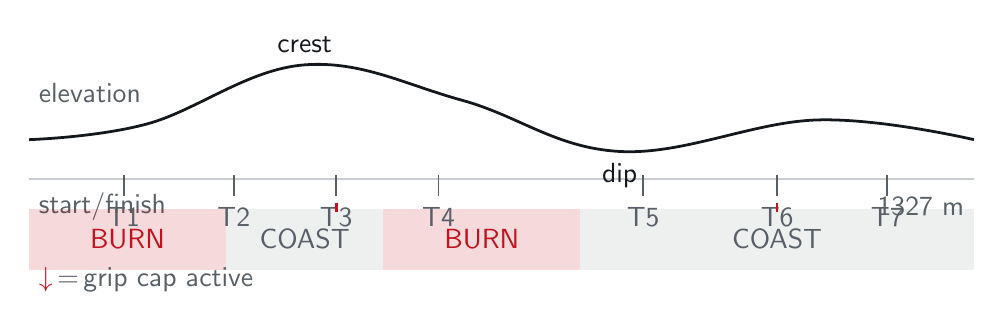
\begin{tikzpicture}[font=\fontsize{10}{11}\selectfont,xscale=1.0]
  %% elevation profile (top strip)
  \draw[draw=mist,line width=0.6pt] (0,0) -- (12,0);
  \node[anchor=west,color=graphite] at (0,-0.35) {\tenpt start/finish};
  \node[anchor=east,color=graphite] at (12,-0.35) {\tenpt\phantom{star}1327 m};
  \draw[draw=ink,line width=1pt]
    plot[smooth,tension=0.65] coordinates
    {(0,0.5)(1.5,0.7)(3.5,1.45)(5.5,1.0)(7.5,0.35)(10,0.75)(12,0.5)};
  \node[color=ink,anchor=south] at (3.5,1.48) {crest};
  \node[color=ink,anchor=north] at (7.5,0.33) {dip};
  \node[color=graphite,anchor=west] at (0,1.1) {elevation};
  %% burn/coast plan (lower strip)
  \fill[accent,opacity=0.16] (0,-1.15) rectangle (2.5,-0.38);
  \fill[graphite,opacity=0.10] (2.5,-1.15) rectangle (4.5,-0.38);
  \fill[accent,opacity=0.16] (4.5,-1.15) rectangle (7.0,-0.38);
  \fill[graphite,opacity=0.10] (7.0,-1.15) rectangle (12,-0.38);
  \node[color=accent] at (1.25,-0.76) {BURN};
  \node[color=graphite] at (3.5,-0.76) {COAST};
  \node[color=accent] at (5.75,-0.76) {BURN};
  \node[color=graphite] at (9.5,-0.76) {COAST};
  %% corner tick-marks T1–T7 with speed-cap indicators
  \foreach \x/\n/\vc in {1.2/T1/0, 2.6/T2/0, 3.9/T3/1, 5.2/T4/0, 7.8/T5/0, 9.5/T6/1, 10.9/T7/0}{
    \draw[color=graphite,line width=0.7pt] (\x,0.05) -- (\x,-0.22);
    \node[color=graphite,anchor=north] at (\x,-0.23) {\n};
    \ifnum\vc=1
      \draw[color=accent,line width=1pt] (\x,-0.30) -- (\x,-0.42);
    \fi
  }
  \node[color=graphite,anchor=west] at (0,-1.28) {\textcolor{accent}{$\downarrow$}\,=\,grip cap active};
\end{tikzpicture}
\caption*{\tenpt\color{graphite}\textbf{Figure~2.}\ Exemplary DP output for Silesia Ring
7-turn representation (Art.~231). Elevation (top) drives the burn/coast plan (bottom);
corner tick-marks T1--T7 show entry positions; red-capped corners (T3, T6) have active
grip-speed constraints $v \leq \sqrt{\mu g r}$. Replace with the surveyed centreline from
the SEM Data \& Telemetry Portal and the computed real-lap plan.}
\end{figure}

% ═══════════════════════ SECTION 5 ════════════════════════════════════
\section{Driver performance on track}
\question{which cues and previews emerge from the strategy, and how they
support the driver's decisions and manoeuvres in specific situations and
edge cases.}

\textbf{Pre-lap preview} (paddock briefing): the plan strip (burn/coast zones
coloured over the track map), target lap time, and energy budget.

\textbf{In-lap cues (one decision at a time):}
a single action card (\textit{``COAST in 50\,m''});
the live speed against a $\pm$1.5\,km/h target band with colour coding
(green~=~on target, amber~=~below, red~=~above);
energy and time deltas versus the current plan (\textit{``$+$2.1\,Wh / $-$3\,s''}).
The existing 0--100 slower/faster driving-hint (channel~$P$) remains as a
fallback mode when no plan is loaded — preserving the graceful-degradation
story.

\textbf{Post-lap debrief (10 seconds):} lap result vs.\ plan and the next
lap's at-most-three changes, e.g.\ \textit{``coast 40\,m earlier into T3 · hold
31\,km/h on S2 · FC set-point $-$10\,W''}.

\begin{tcolorbox}[swisspanel]
\tenpt\color{ink}\textbf{Edge-case playbook}\quad\color{graphite}
\textbf{Rain:} grip coefficient $\mu$ derated 0.70\,$\to$\,0.45;
corner speed caps fall $\approx -25\,\%$; earlier coast cues; WET banner on
both displays. \quad
\textbf{Gusts:} headwind margin added to exposed-straight burn zones. \quad
\textbf{Traffic:} re-time the burn, never defend position. \quad
\textbf{FC over-temperature ($T_{fc}>70\,^{\circ}$C):} derated FC
set-point, alerted by vibration and tone. \quad
\textbf{Link loss:} fail-silent to the last plan; all safety alarms remain
live locally on the phone; the driver always overrides.
\end{tcolorbox}

% ═══════════════════════ SECTION 6 ════════════════════════════════════
\section{Qualitative \& quantitative results improvement}
\question{how the approach balances efficiency, lap time and safety; how the
multi-objective challenge was addressed; expected \% improvement in speed
and energy, with supporting analysis.}

\textbf{Multi-objective solution:} energy is the optimisation objective;
lap time is a hard, priced constraint ($\lambda$ in Eq.~\ref{eq:dp}); safety
constraints are never traded. This is the correct hierarchy: any feasible
plan is valid, the cheapest feasible plan is optimal, and no speed or
energy gain can justify a safety violation.

\textbf{Why the improvement is credible.}
Published work on ultra-efficient vehicles establishes the theoretical gap
between constant-speed and optimal bang--singular--bang driving at
\textbf{15--30\,\%} energy reduction [3--6]; the IEEE 2019 SEM case study
measured $>15\,\%$ improvement over naive driving with a model validated to
3.6\,\% of test data [6]. Our \ex{18\,\%} falls within that range and is
produced by a model fitted to our own logged coast-down and powertrain data
— not datasheets. Confidence column: \textit{H~=~high (physical constraint,
no measurement needed)}, \textit{M~(sim)~=~model-validated simulation result}.

\renewcommand{\arraystretch}{1.18}
\noindent\begin{tabularx}{\linewidth}{@{}L R R R R@{}}
\toprule
\hdr{Metric} & \hdr{Baseline} & \hdr{Optimised} & \hdr{Change} & \hdr{Confidence}\\
\midrule
\hyd\ energy / lap (Wh)     & \ex{52.1}  & \ex{42.7}  & \ex{$-$18.0\,\%} & \ex{M (sim)}\\
Average speed (km/h)         & \ex{27.8}  & \ex{28.2}  & \ex{$+$1.5\,\%}  & \ex{M (sim)}\\
Margin to 35\,min limit (s)  & \ex{$+$4}  & \ex{$+$9}  & \ex{$+$5\,s}     & H\\
Efficiency (\kmM)             & \ex{415}   & \ex{506}   & \ex{$+$21.9\,\%} & \ex{M (sim)}\\
Lap-time variance $\sigma$ (s) & \ex{8}  & \ex{3}     & \ex{$-$63\,\%}   & \ex{M (sim)}\\
\bottomrule
\end{tabularx}
\renewcommand{\arraystretch}{1.0}

\vspace{0.15em}
The reduced lap-time variance ($\sigma$: \ex{8}\,$\to$\,\ex{3}\,s) reflects
the adaptive per-lap loop compensating for weather and model drift —
consistent performance is the hallmark of a strategy that genuinely
closes the loop.

\textbf{Validation protocol at the event (three steps):}
(1)~Practice day, morning: coast-down test on a flat straight — yields
$C_{rr}$ and $C_{dA}$, updates the optimizer.
(2)~Three calibration laps at moderate pace — model error should
converge below 5\,\% by lap~3.
(3)~A/B laps before the scored attempt: one lap at constant speed (baseline),
one following the Lap Coach plan — the measured energy difference is the real
improvement figure. Driver safety cues remain advisory; weather tightens
constraints before any optimisation.

\figslot{28mm}{Back-test: plan speed vs.\ actual speed (distance axis) and cumulative
\hyd\ vs.\ constant-speed baseline, exported from the Lap Coach dashboard after 11 laps.
\textit{Replace with real data from a practice-day MQTT log.}}

% ═══════════════════════ REFERENCES ══════════════════════════════════
\section*{References}
\begin{enumerate}[leftmargin=1.5em,itemsep=1pt,topsep=3pt]
\item Shell Eco-marathon Poland 2026 Official Rules, Chapter~II,
  Art.~225--231 (event format) and Art.~244--247 (off-track awards).
\item ThaiGer TrackControl — telemetry system (team repository):\\
  \url{github.com/D0mm3c/ThaiGerTrackControl}
\item J.-J.~Santin \emph{et~al.}, \emph{The World's Most Fuel Efficient
  Vehicle: Design and Development of PAC-Car~II},
  vdf Hochschulverlag ETH Zürich, 2007.
\item A.~Sciarretta \emph{et~al.}, ``Fundamentals of energy efficient driving
  for combustion engine and electric vehicles: an optimal control
  perspective,'' \emph{Automatica}, vol.~99, pp.~227--243, 2019.
  \url{doi.org/10.1016/j.automatica.2018.10.036}
\item C.~Whitehair \emph{et~al.}, ``Pulse-and-Glide Driving with
  Drivability Constraints: A Pontryagin Approach,''
  arXiv:2012.11435, 2020.
  \url{arxiv.org/abs/2012.11435}
\item J.~Lee \emph{et~al.}, ``Establishing an optimal eco-driving strategy for
  an electric vehicle through testbed simulation — a case study from
  Shell Eco-Marathon 2018,'' in \emph{Proc.\ IEEE VPPC}, 2019.
  \url{doi.org/10.1109/VPPC.2018.8977209}
\item Open-Meteo free weather forecast API (wind, precipitation,
  temperature, pressure for Silesia Ring venue):
  \url{open-meteo.com}
\end{enumerate}

\end{document}

% ═══════════════════════════════════════════════════════════════════════
%  FINAL CHECKLIST (verify before submitting)
% ═══════════════════════════════════════════════════════════════════════
%  [ ] \scaffoldfalse set (line 30 above)                         ✓
%  [ ] \TEAMNAME filled in (not \ph{Team Name})
%  [ ] \TEAMID   filled in (not \ph{Team ID})
%  [ ] \ph{date} replaced with actual submission date
%  [ ] Ran pdflatex TWICE
%  [ ] PDF page count ≤ 10 (open PDF, check last page number)
%  [ ] Team name + ID appear on cover page
%  [ ] Team name + ID appear in header of pages 2, 3, 4, ...
%  [ ] No personal names anywhere in the document
%  [ ] Font size looks ≥ 10 pt throughout (nothing tiny)
%  [ ] Submitted as PDF (not .tex)
% ═══════════════════════════════════════════════════════════════════════
